% !TeX root = ../mat_mod2.tex

\section{
  Стратегии формирования маршрута режущего инструмента
  для типовых заготовок на машиностроительном производстве
}
\label{sect:2.2}
\setcounter{equation}{0}

Стратегия проектирования УП в случае,
когда приоритетными критериями оптимизации УП являются стоимость,
время резки и коэффициент использования материала (КИМ),
значительно отличается по сравнению с оптимизацией
только перемещений инструмента на холостом ходу.
Как отмечалось в первой главе,
применение специальных техник резки
(совмещенный рез, <<цепная>> резка, резка змейкой)
позволяет при проектировании УП сокращать время и стоимость резки.
Ниже описаны специальные методы резки,
которые являются комбинациями вышеописанных специальных способов резки
и позволяют значительно улучшить стоимостные характеристики резки.
Предлагаемые методы резки применимы для типовых
(часто встречающихся геометрических типов)
заготовок на машиностроительных предприятиях.
Эти методы целесообразно реализовать в
виде специализированной подсистемы,
расширяющей штатные возможности САПР (функций САМ модуля)
в автоматическом режиме проектирования УП при построении
маршрута режущего инструмента.
Вместе с тем, при использовании специальных техник
резки необходимо одновременно учитывать соотношения
основных параметров стоимости и времени резки,
к которым относятся
$L_{on}, L_{off}, N_{pt}$.
Например, при использовании <<цепной>> резки
за счет перехода режущего инструмента от одного
контура к другому на рабочем ходу сокращается
количество точек врезок и длина холостого хода,
однако увеличивается значение параметра
$L_{on}$.

При использовании специальных способов резки
с дополнительным резом на рабочем ходу режущего инструмента
для определения эффективности применения специальных
техник резки введем дополнительный параметр
$L_\text{доп}$ -- допустимую длину дополнительного реза
при переходе от одного контура к другому
без выключения режущего инструмента,
который должен удовлетворять следующему соотшению:

\begin{equation}
  L_\text{доп} \leqslant \frac{C_{pt}}{C_{on}}
  .
  \label{l-dop}
\end{equation}

Уменьшение стоимости
$F_{cost}$
от применения специальных способов резки
(например, <<цепная>> резка)
будет происходить только при условии,
когда фактическая длина дополнительного реза
такова, что
\begin{equation}
  L_\text{доп}^\text{факт} < L_\text{доп}
  .
  \label{l-fact-dop}
\end{equation}

При решении задач нерегулярного фигурного раскроя
на практике часто используется прием объединения
фигурных объектов (заготовок)
в группу или <<блок>>.
Под <<блоком>> в этом случае понимается набор заготовок,
положения которых зафиксированы относительно друг друга.
При размещении такой <<блок>> ведет себя как одна заготовка,
то есть все преобразования по перемещению/вращению производятся
одновременно со всеми деталями, входящими в <<блок>>.
Например, все одинаковые прямоугольные треугольники
целесообразно объединять парами в группу, имеющую форму прямоугольника,
с размерами, равными катетам треугольника.
<<Блоки>>, в основном, составляются из однотипных заготовок,
но могут содержать и заготовки различной конфигурации.
Объединение в <<блоки>> актуально в нашем случае.
Ниже будет предложен метод резки для круглых и многоугольных заготовок.

% !TeX root = ../mat_mod2.tex

\subsection{\protect\raggedright
  Стратегии проектирования маршрута режущего инструмента
  для круглых заготовок
}
\label{sect:2.2.1}

Среди часто встречающихся геометрических типов деталей
на машиностроительном производстве можно выделить заготовки,
имеющие внешний контур круглой формы.
Требуемые заготовки можно вырезать с
помощью уже известных способов резки,
например <<цепная>> резка, резка <<по замкнутому контуру>>,
однако применение рассмотренных способов резки не всегда
дает результаты, отвечающие требованиям сокращения стоимости резки.
На основании стратегии объединения однотипных заготовок
в группы разработан специальный способ резки круглых
заготовок с сокращением значений
$L_{off}, N_{pt}$
и в случае без дополнительного реза сокращении значения
$L_{on}$
при одновременном снижении
$F_{cost}$.

На рис.~\ref{3-3}
приведена схема резки трех круглых заготовок
с помощью резки <<по замкнутому контуру>>,
на рис.~\ref{3-1}
-- с помощью предложенного метода резки
с одной точкой врезки без дополнительного реза.

\begin{figure}[h]
  \begin{center}
  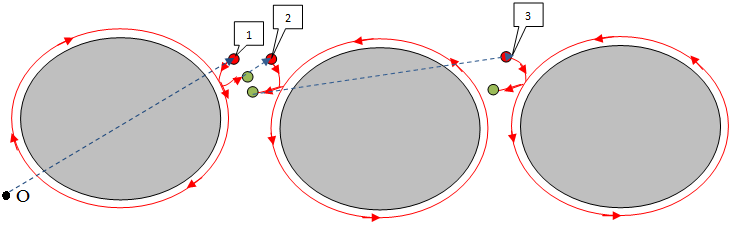
\includegraphics[width=0.9\textwidth]{3-3.png}
  \caption{
    Пример схемы резки трех круглых заготовок
    <<по замкнутому контуру>>
    }
  \label{3-3}
  \end{center}
\end{figure}

На рис.~\ref{3-1}
цифрами от {\it 1} до {\it 5} показана последовательность
резки контуров за один сегмент,
т.е. после врезания в материал режущий инструмент
на рабочем ходу переходит к вырезке участка
под номером {\it 1} первого контура,
затем без дополнительного реза режущая головка
переходит ко второму контуру и вырезает участок
контура под номером {\it 2} и т. д.
В конце режущий инструмент завершает
вырезку трех контуров с одной точкой
врезки по пятому участку первого контура и
переходит к точке выключения.
Следует обратить внимание, что в рассматриваемом
способе резки инструмент переходит от одного контура к
другому на рабочем ходу без дополнительных резов,
за счет чего сокращаются значения основных параметров резки
$L_{on}, L_{off}, N_{pt}$.

\begin{figure}[h]
  \begin{center}
  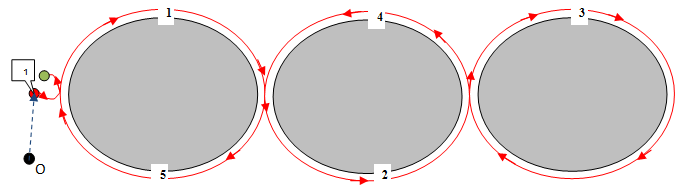
\includegraphics[width=0.9\textwidth]{3-1.png}
  \caption{Пример схемы резки трех круглых заготовок с применением специальной техники резки без дополнительного реза}
  \label{3-1}
  \end{center}
\end{figure}

Однако в результате применения предложенного метода
резки при обработке круглых заготовок в месте <<стыковки>>
контуров возможно образование <<ступеньки>>
(см. рис.~\ref{hiccup}),
что в некоторых случаях может привести к
искажению конечной геометрии и требуемых размеров заготовки.

\begin{figure}[h]
  \begin{center}
  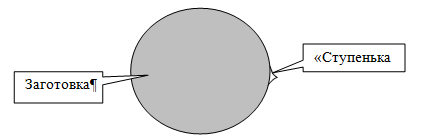
\includegraphics[width=0.7\textwidth]{hiccup.png}
  \caption{Возможная <<ступенька>> при обработке круглых заготовок с помощью специального метода резки}
  \label{hiccup}
  \end{center}
\end{figure}

Как показывает практика,
при обработке круглых заготовок на
машине лазерной листовой резки с ЧПУ размеры <<ступеньки>> незначительны
(достигают десятых-сотых долей мм)
и ее размеры либо попадают в требуемое поле допуска
для соответствующего размера, либо ее можно <<зачистить>>
с помощью дополнительной обработки без искажения геометрии и требуемых размеров.
Также следует отметить, что часто детали,
получаемые после лазерной обработки,
являются заготовками для дальнейших переделов с
припусками на требуемые размеры чертежа,
поэтому допускаются незначительные дефекты,
обработка которых в дальнейшем не приведет к
искажению требуемых размеров и форм конечной детали.

При размещении круглых заготовок в один ряд
либо вдоль оси $Х$,
либо вдоль $Y$
возможно сокращение количества точек врезки до
$N_{pt}=1$
и сведение
$L_{off}$
к величине, равной нулю, если не считать перемещения
режущего инструмента на холостом ходу до точки врезки
для текущего ряда круглых заготовок и от точки выключения
режущего инструмента до следующей точки врезки или нулевой точки
($L_{off} \approx 0$).
В случае размещения круглых заготовок в $n$
рядов при использовании предложенного способа резки
$N_{pt}=n$.

Предложенный на рис.~\ref{3-1}
метод резки круглых заготовок в основном применим для заготовок,
которые можно объединить в один блок и применить
данную специальную технику резки без дополнительного реза.
Однако на практике возникают случаи вырезки круглых заготовок
специальным способом с дополнительным резом,
рис.~\ref{3-extra}.

\begin{figure}[h]
  \begin{center}
  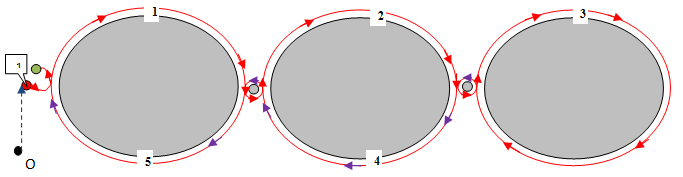
\includegraphics[width=0.9\textwidth]{3-extra.png}
  \caption{Пример схемы резки трех круглых заготовок с применением специальной техники резки с дополнительным резом}
  \label{3-extra}
  \end{center}
\end{figure}

Например, на производстве возникает задача
вырезки круглых заготовок разного габаритного размера,
а также при построении маршрута перемещения режущего инструмента
на машинах термической резки с ЧПУ необходимо выполнение
технологических ограничений термической резки.
В частности, в случае необходимости выполнения условий
сокращения термических деформаций вырезку заготовок с
применением разработанной специальной техники резки
для круглых заготовок необходимо выполнять без изменения обхода контуров.
С этой целью может быть применим способ с дополнительным резом
(рис. \ref{3-extra})
во избежание повышения температуры в процессе резки контуров
в месте стыка деталей из-за острого угла
при переходе от одного контура к другому без изменения
направления обхода и во избежание образования <<ступеньки>>.
Вырезка контуров осуществляется аналогично способу,
приведенному выше
(рис.~\ref{3-3}),
однако при переходе от одного контура к другому
при необходимости возможен дополнительный рез
(при наличии деталей значительно отличающихся по размерам и смещении друг относительно друга).
В свою очередь это может привести к увеличению
$L_{on}$
на величину фактической длины дополнительных резов
$L_\text{доп}^\text{факт}$.
Поэтому в данном способе необходимо вычислять максимально допустимую длину дополнительного реза
$L_\text{доп}$
и
$L_\text{доп}^\text{факт} \leqslant L_\text{доп}$.

На рис.~\ref{3-extra}
красными стрелками показан спроектированный путь
перемещения инструмента на рабочем ходу при прямом обходе контуров,
фиолетовым – обратный ход режущего инструмента
при завершении вырезки трех деталей с
применением специальной техники резки.

Согласно предложенному методу режущая головка
после врезания в материал обходит по часовой
стрелке первый участок контура
(под номером {\it 1}),
после чего меняя направление обхода против
часовой стрелки,
совершает дополнительный рез и
переходит к вырезке участка
(под номером {\it 2})
второго контура по часовой стрелке и т. д.
Пока режущий инструмент не завершит
вырезку полного контура с номером {\it 3},
после чего режущая головка совершает обратный обход
оставшихся невырезанных частей контуров под номерами
{\it 4} и {\it 5}.
Таким образом, можно вырезать заготовки разных размеров,
объединенных в блоки и внутри каждого блока реализовать
вырезку нескольких контуров с помощью одной точки врезки.
При этом дополнительный рез может быть выполнен по дуге
либо по прямой в зависимости от размера внешнего контура заготовок.

С целью оценки эффективности в результате применения
разработанных специальных способов резки рассмотрим
пример резки круглых заготовок двумя вышеописанными
методами на машине лазерной листовой резки
{\it ByStar3015} с ЧПУ.
Для этого были разработаны две раскройные карты,
на которых размещены 69 и 58 заготовок,
имеющих круглый наружный контур.

На рис.~\ref{circles-a}
и~\ref{circles-b}
приведен маршрут резки
круглых заготовок одного размера без дополнительного реза,
на рис.~\ref{circles-c}
и~\ref{circles-d} -- с дополнительным резом.
Полученные результаты сравнивались с результатами
резки <<по замкнутому контуру>> и приведены в
табл.~\ref{circles}.
Расчет был произведен для листового материала
{\it 12Х18Н10Т}
$\Delta$ = 1 и 5 мм.

\begin{figure}
  \begin{center}
  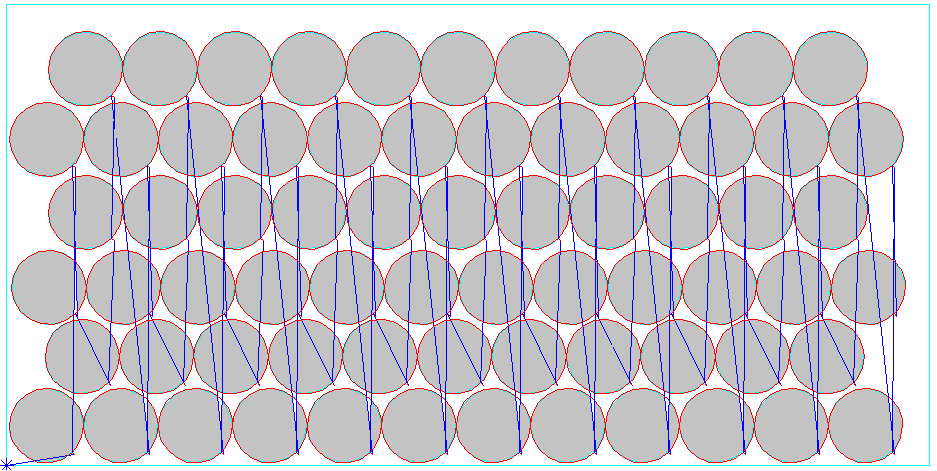
\includegraphics[width=0.9\textwidth]{circles-a.png}
  \caption{
    Пример маршрута резки круглых заготовок
    c~применением резки
    <<по~замкнутому контуру>>
  }
  \label{circles-a}
  \end{center}
\end{figure}

\begin{figure}
  \begin{center}
  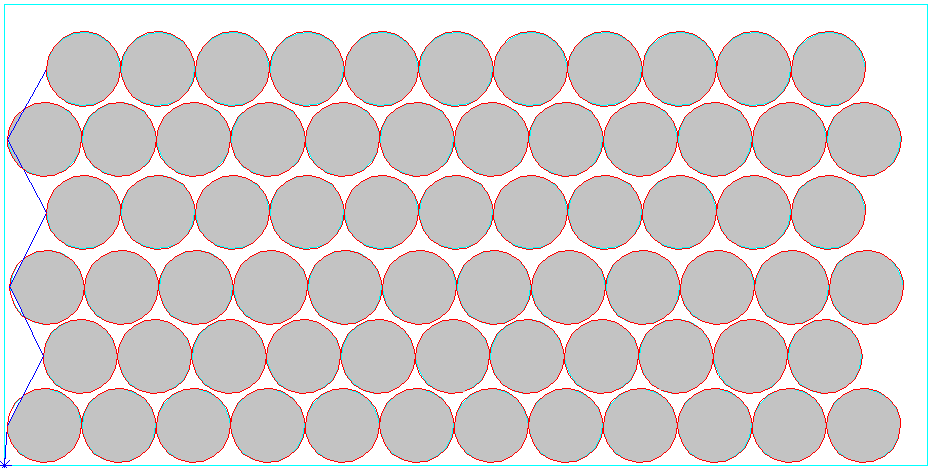
\includegraphics[width=0.9\textwidth]{circles-b.png}
  \caption{
    Пример маршрута резки круглых заготовок
    c~применением метода резки
    без~дополнительного реза}
  \label{circles-b}
  \end{center}
\end{figure}

На рис. \ref{circles-d}
разными цветами обозначены блоки деталей,
для которых реализована резка без дополнительного реза.
В частности, в нижней  части раскройной карты
может быть выделена
группа из 10 круглых заготовок и одного кольца.
Размеры заготовок отличаются незначительно,
поэтому есть возможность реализовать резку блока из 11 деталей с
помощью одной точки врезки и без дополнительного реза.
В  верхней части той же раскройной карты выделен блок из шести деталей,
вырезаемых с одной точкой врезки, при этом заготовки,
выделенные фиолетовым цветом, вырезаются без дополнительного реза,
но при переходе к серым заготовкам меньшего размера необходимо
вырезку осуществить с дополнительным резом.
При этом дальнейшая вырезка трех серых заготовок
осуществляется без дополнительного реза.

\begin{figure}
  \begin{center}
  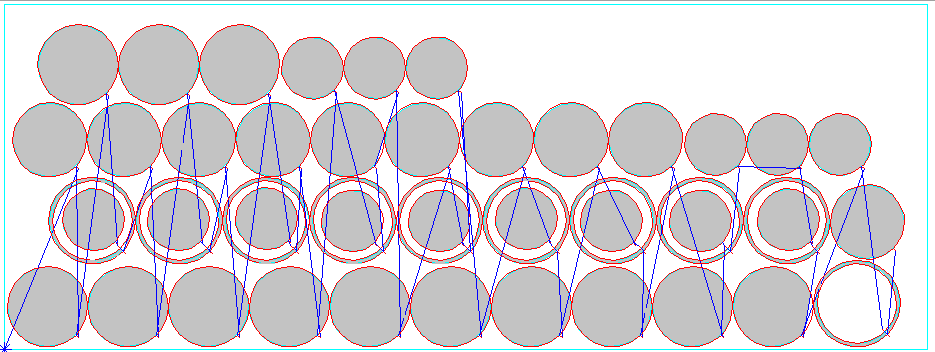
\includegraphics[width=0.9\textwidth]{circles-c.png}
  \caption{
    Пример маршрута резки круглых заготовок разного размера
    c~применением резки
    <<по~замкнутому контуру>>
    }
  \label{circles-c}
  \end{center}
\end{figure}

\begin{figure}
  \begin{center}
  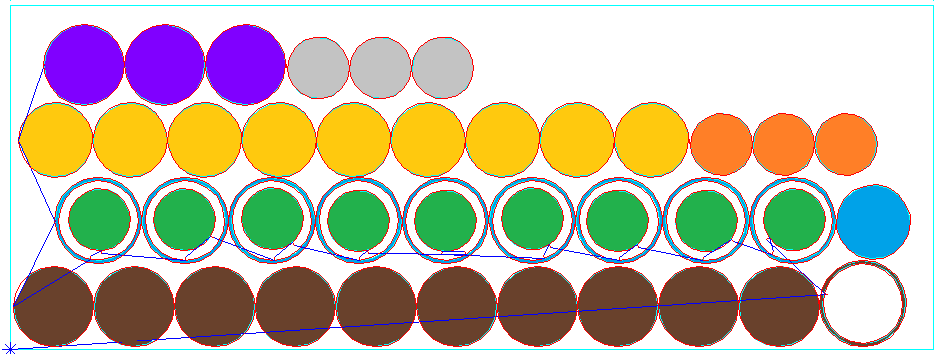
\includegraphics[width=0.9\textwidth]{circles-d.png}
  \caption{
    Пример маршрута резки круглых заготовок разного размера
    c~применением специальной техники резки
    }
  \label{circles-d}
  \end{center}
\end{figure}

\begin{table}
  \caption{
    Результаты расчета стоимость резки раскройного плана
    для~круглых заготовок
    с~применением специальных способов резки
    }
  \label{circles}
  \centering
  \small
  \begin{tabular}{c *{8}{ | c }}
    \hline
    Марка & $\Delta$ & Резка
      & \shortstack{$L_{on}$, \\ м}
      & \shortstack{$L_{off}$, \\ м}
      & $N_{pt}$
      & \shortstack{$F_{cost}$,\\ руб}
      & \%
      & \shortstack{$L_\text{доп}^\text{факт}$,\\ м} \\
    \hline
    \multirow{8}{*}{\rotatebox{90}{12Х18Н10Т}} & \multirow{4}{*}{1 мм} & Стандартная & 54,7 &	43,07	& 69 & 1552,92 & \multirow{2}{*}{15,6} &	\multirow{2}{*}{--} \\
    & & Без доп. реза & 52.02 &	0.7 & 6 & 1310.05 \\
    & & Стандартная   & 46.14 & 18.78 & 58 & 1302.08 & \multirow{2}{*}{6.88} & \multirow{2}{*}{0.16} \\
    & & С доп. резом  & 46.3  & 5.43  & 23 & 1212.43 \\
    & \multirow{4}{*}{5 мм} & Стандартная & 54.7 &	43.07	& 69 & 12154.8 & \multirow{2}{*}{14.3} &	\multirow{2}{*}{--} \\
    & & Без доп. реза & 52.02 &	0.7 & 6 & 10417.2 \\
    & & Стандартная   & 46.14 & 18.78 & 58 & 10241.6 & \multirow{2}{*}{6.2} & \multirow{2}{*}{0.16} \\
    & & С доп. резом  & 46.3  & 5.43  & 23 & 9607.08 \\
    \hline
  \end{tabular}
\end{table}

По результатам анализа приведенных
в~табл.~\ref{circles}
данных, можно сделать следующие выводы.

\begin{enumerate}
\item
Применение специального метода резки круглых заготовок
без дополнительного реза
(рис.~\ref{circles-b})
приводит к сокращению количества точек врезок до 90 \%
и длины перемещений инструмента на холостом ходу до 98 \%
по сравнению с резкой по <<замкнутому контуру>>.
При проведении ряда экспериментов в среднем значение $N_{pt}$
сокращается на 60 \%, значение $L_{off}$ на 65 \%.
При этом стоимость обработки раскройной карты в среднем сокращается на 15 \%.

\item
Применение резки с дополнительным резом
(рис.~\ref{circles-d})
приводит в среднем к сокращению количества точек врезок на 60 \%,
а длины перемещений инструмента на холостом ходу сокращается на 70 \%
по сравнению с резкой <<по замкнутому контуру>>.
В свою очередь стоимость обработки сокращается на 7 \%.
При этом следует отметить,
что по причине наличия внутренних контуров
наблюдается снижение эффективности применения
предложенных технологий.

\item
В случае применения резки с дополнительным резом необходимо рассчитать
$L_\text{доп}^\text{факт}$.
и
$L_\text{доп}$
согласно (\ref{l-dop}) и (\ref{l-fact-dop}).
\end{enumerate}

% !TeX root = ..

\subsection{
  Стратегии проектирования маршрута режущего инструмента
  для многоугольных заготовок
}
\label{sect:2.2.2}

В машиностроительном производстве
при раскрое листового материала с помощью машин лазерной резки с ЧПУ
к наиболее часто встречающимся геометрическим
типам заготовок,
помимо круглых внешних контуров,
относят также многоугольные заготовки --
часто выпуклые симметричные многоугольники с отверстиями различной формы.
К отдельной группе можно отнести треугольные и прямоугольные заготовки.
Следует отметить, что прямоугольные заготовки целесообразно обрабатывать
с помощью совмещенного реза.
Касательно остальных многоугольных (в т. ч. треугольных)
заготовок применение совмещенного реза неэффективно,
т. к. обычно с помощью одной точки врезки удается вырезать обычно две заготовки.
Также неэффективны другие специальные способы резки
(например, <<цепная>> резка или резка змейкой),
т. к. применение выделенных способов приводит к
сокращению количества точек врезок,
но
$L_{on}=\mathrm{const}$
что,
в свою очередь,
повышает время
$T_{cut}$
и стоимость раскроя
$F_{cost}$.
Поэтому возникает необходимость в разработке
новых специальных способов резки для выделенной группы заготовок.

В отдельную группу выделим треугольные заготовки,
для листовой резки которых на машине лазерной резки с ЧПУ
применим мультиконтурную резку,
соединяющую совмещенный рез и резку змейкой.
На рис.~\ref{6-6}
приведена схема резки шести треугольных заготовок
одного размера с помощью резки <<по замкнутому>> контуру, при этом
$N_{pt}=6$
(цифрами {\it 1--6}
обозначена последовательность резки).

\begin{figure}[H]
  \centering
  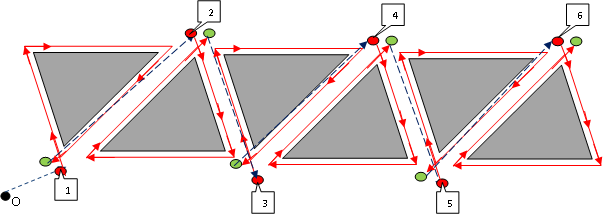
\includegraphics[width=0.9\textwidth]{6-6.png}
  \caption{
    Схема резки шести треугольных заготовок
    с помощью резки
    <<по~замкнутому контуру>>
  }
  \label{6-6}
\end{figure}

На рис.~\ref{6-1} приведена схема резки тех же шести
треугольных заготовок, при этом
$N_{pt}=1$.
Цифрами {\it 1--13} обозначена последовательность
резки контуров в одном сегменте,
т. е. после врезания в материал режущий инструмент
на рабочем ходу переходит к вырезке участка под номером {\it 1}
первого контура,
затем без дополнительного реза режущая головка
переходит ко второму контуру и вырезает участок под номером
{\it 2} и т. д.
В конце режущий инструмент завершает вырезку шести контуров
с одной точкой врезки по {\it 13} участку и переходит к
точке выключения инструмента.
Следует обратить внимание, что в рассматриваемом способе
резки инструмент переходит от одного контура к другому
на рабочем ходу с совмещенным резом,
за счет чего сокращается количество точек врезки $N_{pt}$,
расстояние перемещений инструмента на рабочем $L_{on}$
и холостом  $L_{off}$ ходах.

\begin{figure}[H]
  \centering
  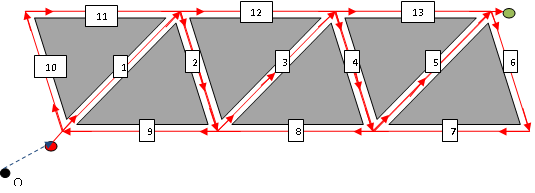
\includegraphics[width=0.9\textwidth]{6-1.png}
  \caption{
    Схема резки шести треугольных заготовок
    с помощью специального способа резки
  }
  \label{6-1}
\end{figure}

Способ резки, предложенный
на~рис.~\ref{6-1},
применим для групп треугольных заготовок одного типоразмера,
расположенных в два ряда.
При этом если количество рядов больше двух,
то создаются еще блоки заготовок,
каждый из которых включает в себя по два ряда треугольных заготовок.
Переход режущего инструмента от одного блока к другому
осуществляется с помощью холостого хода.
Внутри каждого блока реализована резка заготовок с одной точкой врезки.

В случае раскроя листового материала треугольными
заготовками можно спроектировать маршрут режущего
инструмента без холостого хода,
для этого треугольные заготовки необходимо
размещать согласно рис.~\ref{3-10}.
Основное условие непрерывной резки нескольких
заготовок заключается в том,
что общее количество пересекающихся ребер у
любой вершины треугольника должно быть четным.
Или, с точки зрения теории графов,
у каждой вершины
должно быть четное количество ребер.
В обратном случае непрерывную резку заготовок
с помощью одной точки врезки не осуществить
без дополнительных резов.
Например, как видно из рис.~\ref{3-10},
общее количество обозначенных цифрами
{\it 1, 2, 4, 5, 7} и {\it 8} ребер равно 6.

\begin{figure}[H]
  \centering
  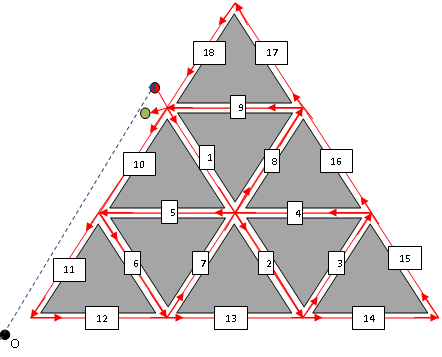
\includegraphics[width=0.8\textwidth]{3-10.png}
  \caption{
    Схема резки девяти треугольных заготовок
    с~помощью мультиконтурной~резки
  }
  \label{3-10}
\end{figure}

Цифрами {\it 1 -- 18} обозначена последовательность
резки контуров за один сегмент,
т. е. после врезания в материал режущий инструмент
на рабочем ходу переходит к вырезке участка
первого контура
(под номером {\it 1}),
затем без дополнительного реза режущая
головка переходит ко второму контуру и
вырезает участок под номером {\it 2} и т. д.
В конце режущий инструмент завершает
вырезку девяти контуров с одной точкой врезки
по {\it 18} участку и переходит к точке выключения инструмента.
Следует обратить внимание, что в рассматриваемом способе
резки инструмент переходит от одного контура к
другому на рабочем ходу с совмещенным резом,
за счет чего сокращается количество точек врезки $N_{pt}$,
расстояние перемещений инструмента на рабочем ходу  $L_{on}$,
при этом
$L_{off} \approx 0$.
Холостой переход осуществляется
только при переходе режущего инструмента
от нулевой точки до точки врезки и от
точки выключения инструмента до нулевой точки.
Способом, приведенным на рис. \ref{3-10},
можно размещать большое количество
треугольных заготовок, при этом всегда $N_{pt}=1$
и $L_{off} \approx 0$.

Предложенные выше методы резки применимы для любых треугольников.

Обработку пятиугольных заготовок из листового материала
на машине лазерной резки с ЧПУ также можно осуществить
предложенным методом, приведенным
на~рис.~\ref{6-1}
с помощью мультиконтурной резки,
объединяющей совмещенный рез и резку змейкой.
На рис.~\ref{5-6}
приведена схема резки <<по~замкнутому>> контуру
шести пятиугольных заготовок,
при этом $N_{pt}=6$.

\begin{figure}[H]
  \centering
  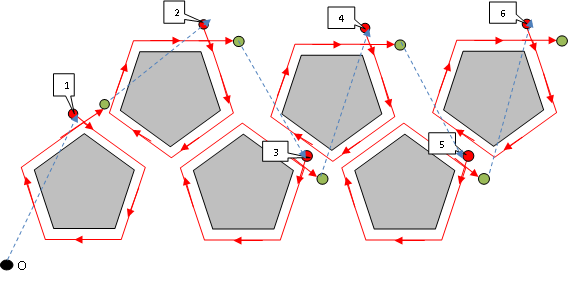
\includegraphics[width=0.9\textwidth]{5-6.png}
  \caption{
    Схема резки <<по замкнутому контуру>>
    шести пятиугольных заготовок
  }
  \label{5-6}
\end{figure}

На рис.~\ref{5-1}
предложена схема резки тех же шести
пятиугольных заготовок за один сегмент, при этом
$N_{pt}=1$
и $L_{off} \approx 0$.
С ее помощью
можно осуществлять резку по ребрам многоугольников,
соблюдая последовательность и направление резки каждого ребра.
Ход реза обозначен цифрами {\it 1--25}.
Инструмент перемещается на холостом ходу от
начальной точки положения инструмента
(точки {\it О})
до точки врезки, после чего осуществляется непрерывная резка всех ребер,
начиная с {\it 1},
без дополнительных резов за один сегмент.
После того как режущий инструмент частично вырежет
первый контур по четырем ребрам (с {\it 1} по {\it 4}),
он переходит к ребру {\it 5} и начинает вырезать
второй контур, последовательно вырезая с {\it 6} по {\it 9} ребра.
При вырезке {\it 9} ребра будут окончательно
вырезаны первый и второй контуры.
Аналогично можно вырезать оставшиеся контуры,
после чего инструмент переходит в точку выключения инструмента.

Как видно из рис.~\ref{5-1},
за счет применения совмещенного реза сокращается $L_{on}$,
за счет отсутствия холостых переходов
$L_{off} \approx 0$
и $N_{pt}=1$
при одновременном сокращении общего времени
и стоимости резки заготовок из листового
материала на машинах лазерной резки с ЧПУ.
Предложенный способ резки применим для любых выпуклых пятиугольников.

\begin{figure}[H]
  \centering
  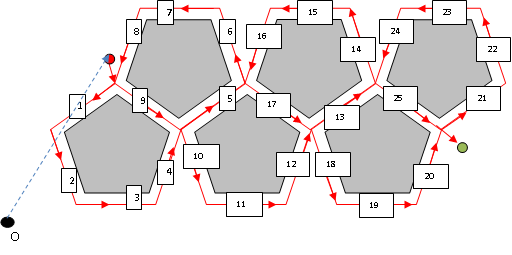
\includegraphics[width=0.9\textwidth]{5-1.png}
  \caption{
    Схема резки шести пятиугольных заготовок
    с применением мультиконтурной резки
  }
  \label{5-1}
\end{figure}

В случае обработки четырехугольных заготовок
целесообразно применять совмещенный рез
либо технологию, предложенную
на~рис.~\ref{5-1},
при условии, что общее количество ребер,
пересекающихся в любой внутренней вершине, будет четным.
В последнем случае значения
$N_{pt}$
и $L_{off}$
при использовании разработанного способа резки будут,
как правило, ниже, чем при совмещенном резе.
Но данный способ резки не всегда применим
с точки зрения снижения КИМ.

В общем случае при резке любых многоугольных
заготовок для случая,
когда количество пересекающихся ребер у вершин
(в частности внутренних) нечетно,
то предложенный способ резки реализуем с
дополнительным резом, либо с добавлением точек врезки.
Следует обратить внимание на то,
что при мультиконтурной резке многоугольников с
дополнительным резом значение
$L_\text{доп}^\text{факт}$
также как и для треугольников должно удовлетворять условию
$L_\text{доп}^\text{факт} \leqslant L_\text{доп}$,
рассчитанному по (\ref{l-fact-dop}),
а иначе значения целевых функций (\ref{cutting-time})
и (\ref{cutting-cost})
окажутся больше значений,
получаемых  при резке <<по замкнутому контуру>>.
На рис.~\ref{5-extra}
для любой вершины количество пересекающихся ребер нечетно,
поэтому резка контуров возможна только с дополнительным резом.

\begin{figure}[H]
  \centering
  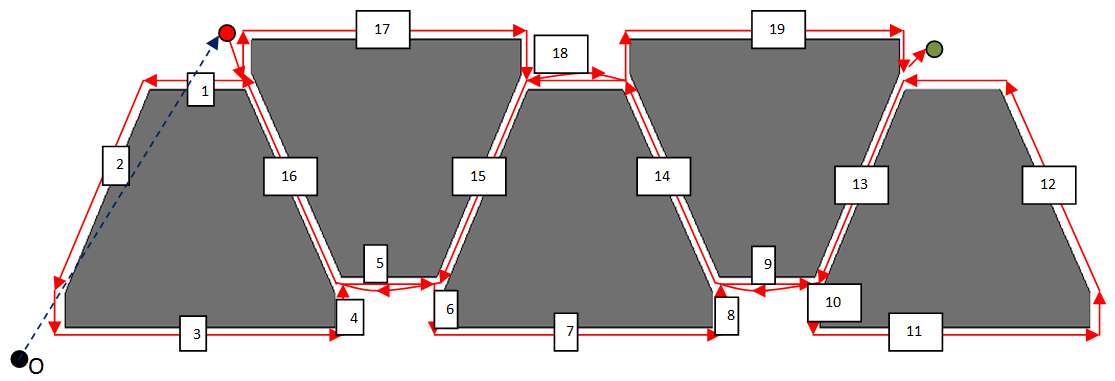
\includegraphics[width=0.9\textwidth]{5-extra.png}
  \caption{
    Схема резки пяти заготовок
    с помощью мультиконтурной резки
    с~дополнительным резом
    }
  \label{5-extra}
\end{figure}

Цифрами {\it 1--19} обозначена последовательность обхода ребер
пяти заготовок.
Режущий инструмент на холостом ходу переходит
из начальной точки в точку врезки,
после чего по эквидистантому контуру
осуществляется частичная вырезка первого
контура по ребрам {\it 1--4},
затем вырезается ребро {\it 5} второй заготовки и т. д.,
пока окончательно не будут вырезаны пять заготовок по ребрам
{\it 6--19}.
По причине наличия дополнительных резов рабочая
длина перемещения режущего инструмента может увеличиться по сравнению с $L_{on}$,
полученной в результате применения резки <<по замкнутому контуру>>,
поэтому актуален вопрос проверки неравенства
$L_\text{доп}^\text{факт} \leqslant L_\text{доп}$.
В результате применения предложенного на рис.~\ref{5-extra}
специального метода резки
$N_{pt}=1$
и $L_{off} \approx 0$.

Рассмотрим пример раскроя листового материала
{\it 12Х18Н10Т}
($\Delta$ = 1--8 мм)
многоугольными заготовками на машине лазерной резки с ЧПУ.
Для этого разработаны две раскройные карты с одинаковым количеством,
видом и размерами деталей,
для которых спроектирован маршрут перемещения
режущего инструмента в САПР <<Сириус>> с
применением резки <<по замкнутому контуру>>
(рис.~\ref{multi-a})
и специальной техники резки для многоугольных заготовок
(рис.~\ref{multi-b}).
Маршрут резки в обоих случаях
начинается в левом нижнем углу листа.

Полученные результаты, которые содержат значения
$L_{on}$, $N_{pt}$, $L_{off}$, $T_{cut}$ и $F_{cost}$
для каждой раскройной карты, приведены
в~табл.~\ref{polygons}
на стр.~\pageref{polygons}.

\begin{figure}[H]
  \centering
  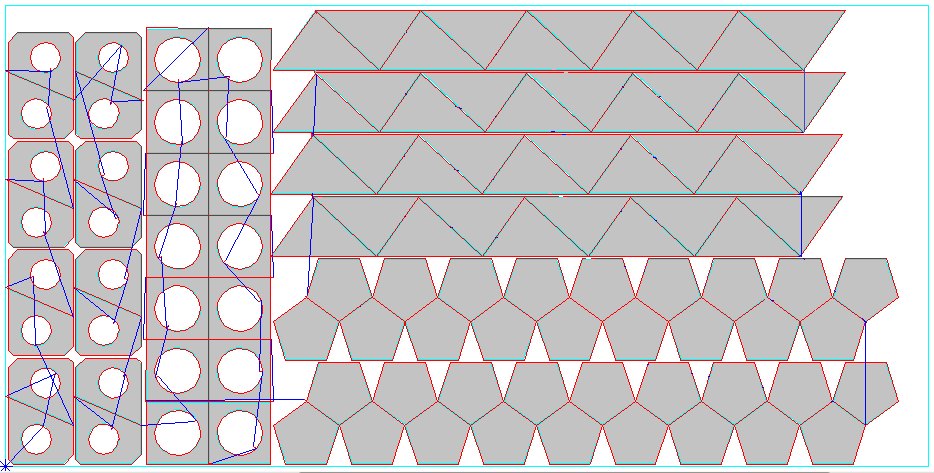
\includegraphics[width=0.9\textwidth]{multi-a.png}
  \caption{
    Схема раскройной карты
    с применением мультиконтурной резки
    для~многоугольных заготовок
  }
  \label{multi-a}
\end{figure}

\begin{figure}[H]
  \centering
  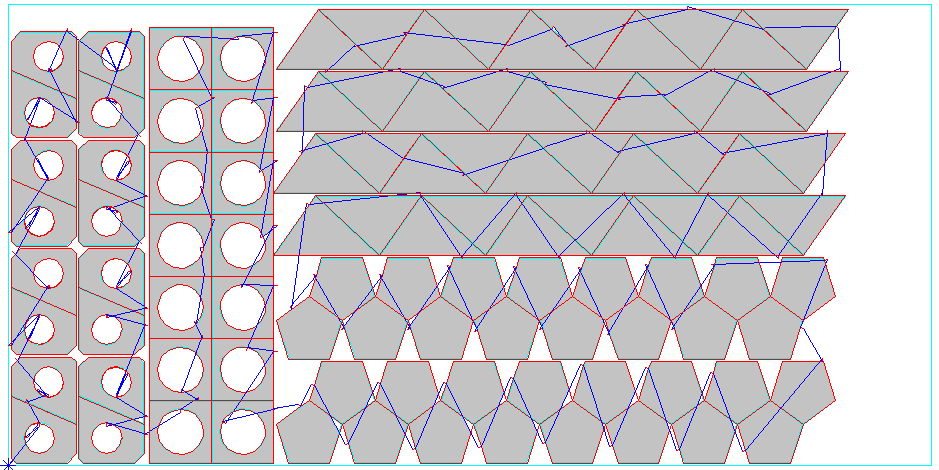
\includegraphics[width=0.9\textwidth]{multi-b.png}
  \caption{Схема раскройной карты с применением резки <<по замкнутому контуру>>}
  \label{multi-b}
\end{figure}

Применение предложенных специальных методов резки
приводит к значительному сокращению значений
$N_{pt}$, $L_{on}$ и $L_{off}$
в сравнении со стандартной техникой резки
соответственно до 70 \%, 27 \% и 67 \%
при одновременном сокращении времени
$T_{cut}$
и стоимости лазерной резки
$F_{cost}$ до 36 \%.
Как показывает практика применения
предложенных методов резки при проектировании
УП в реальном производственном процессе,
в среднем значения параметров
$L_{on}$, $N_{pt}$  и $L_{off}$
сокращаются на 3 \%, 60 \% и 65 \%
соответственно при одновременном снижении
$F_{cost}$
на 10--20 \%
по сравнению с резкой <<по замкнутому контуру>>.
Как видно из табл.~\ref{polygons}
с увеличением толщины обрабатываемого материала
сокращается эффективность предложенных специальных способов резки.

\begin{table}[H]
  \caption{
    Результаты расчета стоимости резки раскройного плана
    для~многоугольных заготовок
    }
  \label{polygons}
  \centering
  \begin{tabular}{c *{7}{|c}}
    \hline
    Марка & $\Delta$ & Резка &
      \shortstack{$L_{on}$, \\ м} &
      \shortstack{$L_{off}$, \\ м} &
      $N_{pt}$ &
      \shortstack{$F_{cost}$, \\ руб} &
      \% \\
    \hline
    \multirow{2}{*}{12Х18Н10Т} & \multirow{2}{*}{1 мм} & Стандартная & 101,85 & 26,92 & 163 & 2956,14 & \multirow{2}{*}{36,0} \\
    & & Специальная & 74,73 & 8,90 & 51 & 1901,4 \\
    \multirow{2}{*}{12Х18Н10Т} & \multirow{2}{*}{3 мм} & Стандартная & 101,85 &	26,92 & 163 & 9170,09 & \multirow{2}{*}{36,5} \\
    & & Специальная & 74,73 & 8,90 & 51 & 5823,10 \\
    \multirow{2}{*}{12Х18Н10Т} & \multirow{2}{*}{5 мм} & Стандартная & 101,85 & 26,92 & 163 & 23262,44 & \multirow{2}{*}{32,2} \\
    & & Специальная & 74,73 & 8,90 & 51 & 15768,17 \\
    \multirow{2}{*}{12Х18Н10Т} & \multirow{2}{*}{8 мм} & Стандартная & 101,85 & 26,92 & 163 & 94070,86 & \multirow{2}{*}{29,7} \\
    & & Специальная & 74,73 & 8,90 & 51 & 66121,93 \\
    \hline
  \end{tabular}
\end{table}

Таким образом, можно сделать следующие выводы.

\begin{enumerate}
\item
Применение специальных методов резки
для различных многоугольных заготовок возможно
без дополнительных резов между заготовками при условии,
что количество пересекающихся ребер у вершин
(в частности, внутренних) четно.
В остальных случаях резка разработанным
способом возможна с дополнительным резом,
либо с увеличением числа точек врезки.
Предложенные методы базируются на известных методах резки
(змейкой и совмещенный рез),
за счет этого значительно сокращаются
значения основных параметры
$L_{on}$, $N_{pt}$  и $L_{off}$
при одновременном снижении
$T_{cut}$
и
$F_{cost}$.

\item
В зависимости от типа заготовок,
наличия или отсутствия отверстий в деталях
количество точек врезки может снизиться до
$N_{pt}=1$,
при этом
$L_{off} \approx 0$.
В рассмотренных примерах значения
$N_{pt}$, $L_{off}$ и $L_{on}$
максимально сокращаются соответственно до 70 \%, 67 \% и 27 \%
при одновременном сокращении
$T_{cut}$
и
$F_{cost}$
до 36 \%.
В среднем значение $F_{cost}$ снижается на 10--20 \%.

\item
При применении предложенных специальных способов резки
для многоугольных деталей с дополнительным резом
необходимо вычислить значение
$L_\text{доп}^\text{факт}$:
$L_\text{доп}^\text{факт} \leqslant L_\text{доп}$.
В противном случае значение
$L_\text{доп}$
может оказаться больше значения
$L_{on}$,
полученное при резке <<по замкнутому контуру>>,
что,
в свою очередь,
может привести к увеличению значений целевых функций
$T_{cut}$
и
$F_{cost}$.

\item Эффективность применения предложенных способов резки
сокращается при увеличении толщины обрабатываемого материала.
\end{enumerate}

Отметим, что
предложенные способы применения специальных техник резки и
формирование групп однотипных заготовок на этапе
проектирования раскроя листовых материалов на фигурные заготовки,
среди которых присутствуют круглые и многоугольные,
можно интерпретировать как методы формирования наборов базовых сегментов
(а в дискретном случае – мегаполисов)
для последующего решения задач оптимизации класса
{\it GSCCP}
средней и большой размерности.
Это создает,
в свою очередь,
предпосылки  для разработки эффективных методов
решения интегрированной задачи раскроя и маршрутизации,
для которой целевая функция стоимости складывается
из стоимости использованного материала для раскроя
и стоимости процесса резки
$
F_{cost}=
L_{on} \cdot C_{on} +
L_{off} \cdot C_{off} +
N_{pt} \cdot C_{pt}
$.

